\section[Das Sommerfest der Fachschaft]{Die Physik braucht ein Sommerfest!\\Das Sommerfest der Fachschaft}
\begin{multicols*}{2}

\textbf{Was wäre ein Sommer ohne Sommerfest?
	Nicht auszudenken!
	Deswegen (und nicht etwa aus Freude am Feiern und Organisieren) veranstaltet die Fachschaft Physik dies seit Jahren.}

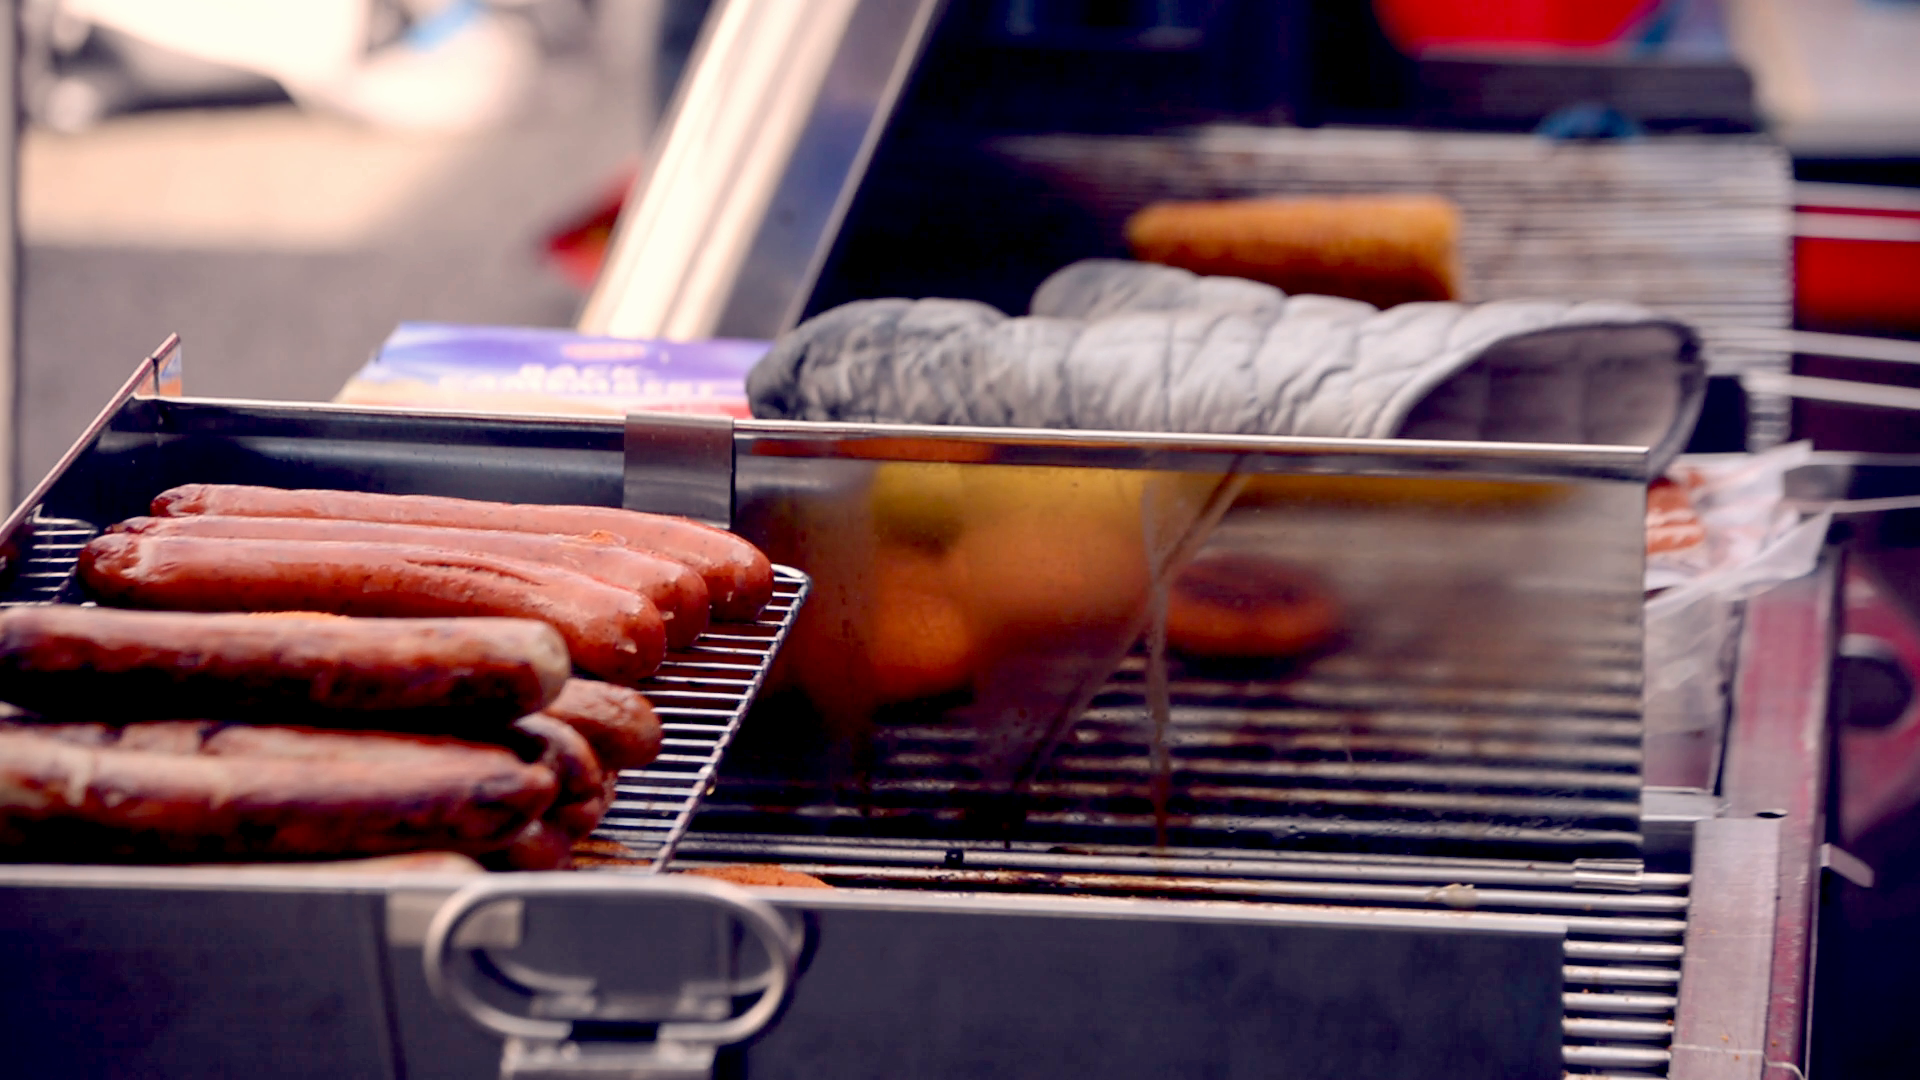
\includegraphics[width=\columnwidth]{res/sommerfest_grill.png}

Um euch einen Überblick geben zu können, was auch euch im Sommer des nächsten Jahres erwarten wird, hier der Bericht diesen Jahres:

Auch in diesem Jahr kam das Sommerfest der Fachschaft~Physik bei allen Beteiligten gut an und war ein großer Erfolg.
Insgesamt kamen ungefähr \num{3,2e2}~Leute (Zahl grob durch Autor geschätzt, kann von realen Gegebenheiten abweichen) und genossen das umfangreiche Rahmenprogramm bei Bier, Musik und 'was leckerem vom Grill.

Pünktlich um 11:00~Uhr wurde der Grill angezündet und so konnten die ersten Besucher als Mittagessen einen herzhaften Grillkäse und eine gute Bratwurst genießen.

Durch eine Fragestunde zum Erasmus-Programm mit ehemaligen Erasmus-Studenten und dem Erasmus-Beauftragten, Prof.\ Dr.\ Kappes, hatte der Tag auch eine fast schon bildende Komponente.

Die gleißende (aber eigentlich ganz angenehm warme) Sonne ließ die Teams des Volleyballturniers nicht davon abhalten, die lang ersehnten Spiele um 13:00~Uhr auszuführen, und so trafen die Mannschaften im K.\,O.-System aufeinander und boten sich einen harten, aber fairen Kampf um den Sieg.
Von der Vorgruppe über Viertel- und Halbfinale bis hin zum Finale konnte jedes Team sein Können unter Beweis stellen.

Wenn den Teams nach den Spielen allzu warm war, konnten sie, ebenso wie alle anderen Besucher natürlich auch, zu jeder vollen Stunde von unserem selbstgemachten Stickstoffeis kosten -- ein beim Herstellen visuelles und beim Verzehr kulinarisches Highlight des Sommerfests. 

Um 16:15~Uhr wurde das von vielen herbeigefieberte Physiker-Duell veranstaltet.
Bei diesem nach dem Vorbild des alten "Familien-Duells" und des neuen "Codename" konzipierten Spiel trafen drei Arbeitsgruppen des Fachbereiches Physik aufeinander und stellten sich den Fragen des Moderators Fernando.

Zuvor wurden "100~Physiker" (Physikstudenten) gefragt und es galt natürlich, die meistgegebenen Antworten zu erraten.
In diesem Jahr traten die Arbeitsgruppen von Professor Kuhn, Krüger und Schuck in einem unfassbar spannenden Duell gegeneinander an, bei dem schließlich die AG um Professor Kuhn den Sieg erlangte.

Unterlegt wurde der ganze Tag von Musik, die mit einem breiten Spektrum an musikalischen Meisterwerken eine perfekte Kulisse schuf. In diese Kulisse fügte sich in diesem Jahr hervorragend eine Hüpfburg ein, welche sich für ausgelassenes Hüpfen genauso wie für ihrer luftmatratzenähnlichen Gemütlichkeit einer großen Beliebtheit erfreute.

Da der Abend nach hinten hin offen gehalten wurde, blieben einige noch zum Marshmallows grillen am Lagerfeuer und ließen
den Abend so ausklingen.

Ein langes und erfolgreiches Sommerfest war nun beendet und sucht im nächsten Jahr einen würdigen Nachfolger.
Dann natürlich auch mit euch, die ihr jetzt schon mal herzlichst zum größten, öffentlichen seiner Art am Fachbereich eingeladen seid.
Besonders für das Volleyballturnier werden natürlich weitere starke Gegner gesucht!
\fibelsig{Benedikt}
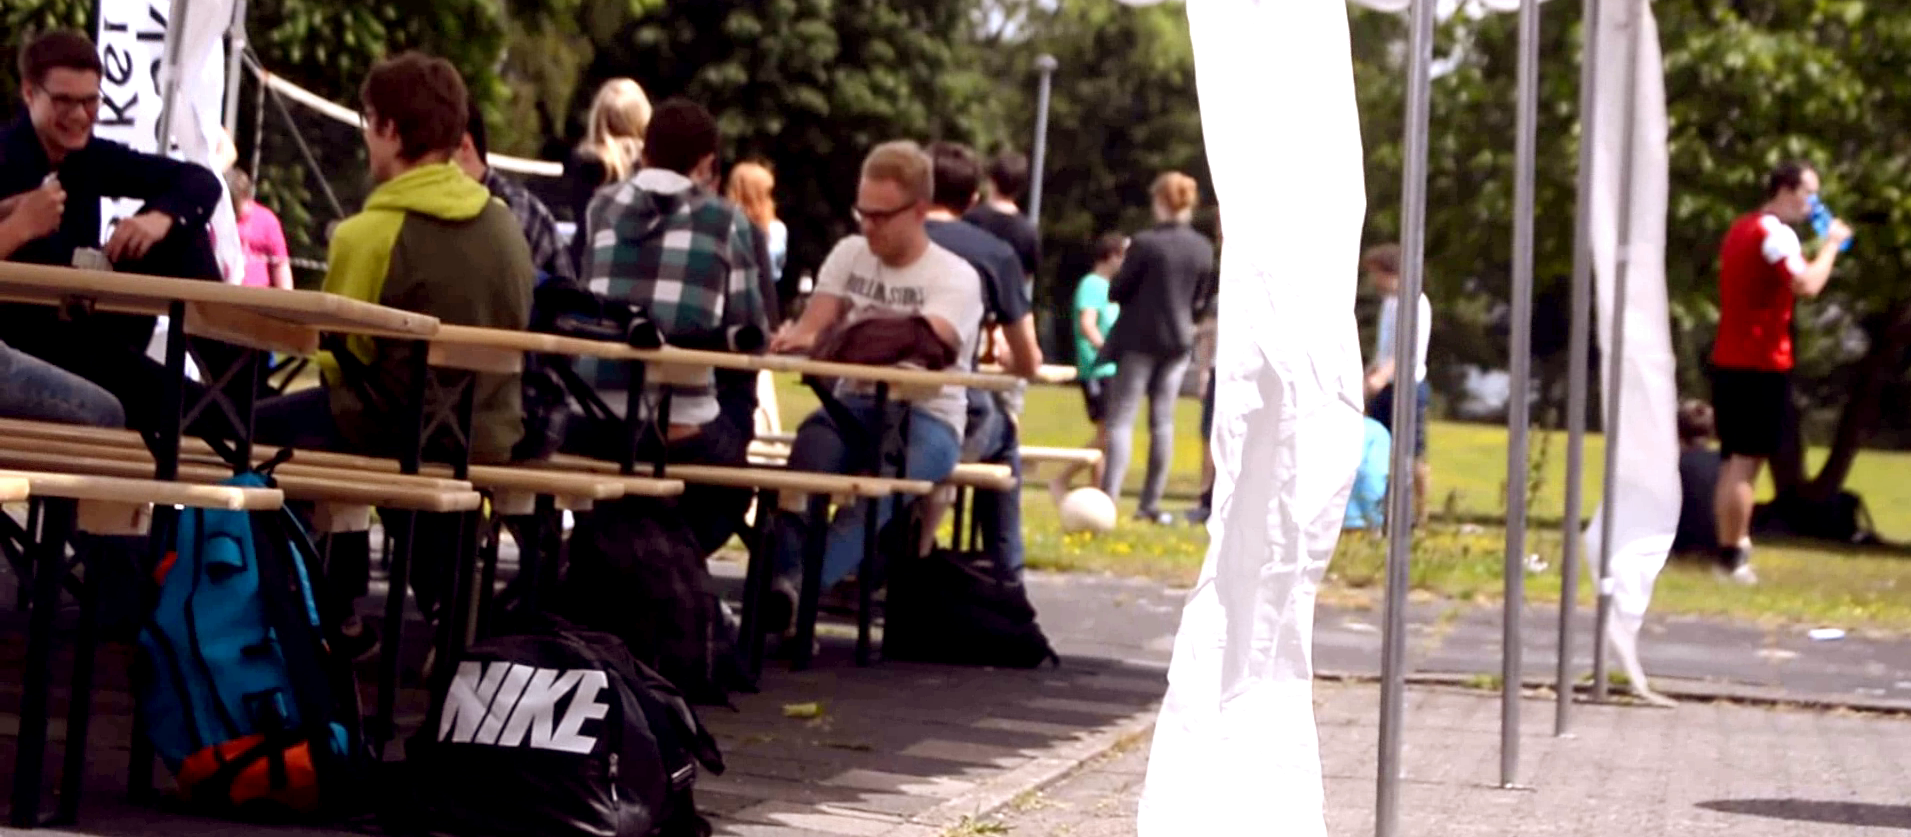
\includegraphics[width=\columnwidth]{res/sommerfest_zelt_cropped}
\end{multicols*}
